\documentclass[aspectratio=169]{ctexbeamer}
\usepackage[T1]{fontenc}
\usepackage{mathtools}
\usepackage{tikz}
\usepackage{booktabs}
\usepackage{caption}
\usepackage{outlines}
\usepackage{graphicx}
\usepackage{float}
\usepackage{amsthm}
\usepackage{tabularray}
\usepackage{minted}
\usepackage{hyperref}
\usepackage{underscore}
\usepackage{cleveref}
\RequirePackage{pgfgantt}
\usetheme[
    progressbar=frametitle,
    numbering=fraction,
    subsectionpage=progressbar,
    titleformat title=smallcaps,
    titleformat subtitle=smallcaps,
    titleformat section=smallcaps,
    titleformat frame=smallcaps]{metropolis}

\UseTblrLibrary{booktabs}

\DeclarePairedDelimiter{\set}{\{}{\}}
\DeclarePairedDelimiter{\paren}{(}{)}
\graphicspath{ {./images/} }

\newcounter{fullrefcounter}
\newcommand*{\fullref}[1]{%
\addtocounter{fullrefcounter}{1}%
\label{--ref-\thefullrefcounter}%
\ifthenelse{\equal{\getpagerefnumber{--ref-\thefullrefcounter}}{\getpagerefnumber{#1}}}
  {
    \hyperref[{#1}]{\Cref*{#1} \nameref*{#1}}
  }
  {% false case
    \hyperref[{#1}]{第 \pageref*{#1} 页 \Cref*{#1} \nameref*{#1}}
  }
}
\definecolor{bjutblue}{HTML}{429ABF}
\setbeamercolor{palette primary}{bg=bjutblue}

\setbeamertemplate{footline}{
    \hbox{%
    \begin{beamercolorbox}[wd=\paperwidth,ht=3ex,dp=1.5ex,leftskip=2ex,rightskip=2ex]{page footer}%
        \usebeamerfont{title in head/foot}%
        \hfill
        \begin{tblr}{
            width=.8\linewidth,
            colspec={X[l]X[c]X[r]}
        }
            \insertshorttitle &
            \ifx\insertsection\empty
            \else
            \insertsection{}
                \ifx\insertsubsection\empty\else
                    -- \insertsubsection
                \fi
            \fi &
            \insertframenumber{} / \inserttotalframenumber
        \end{tblr}
        \hfill{}
    \end{beamercolorbox}}%
}

\title{BM4KG技术选型讨论}
\author{卢雨轩}
% \date{\today}
\ctexset{
    today = small,
    figurename = 图,
    contentsname = 目录,
    tablename = 表,
}

\begin{document}

\maketitle
\begin{frame}{主要内容}
    \setbeamertemplate{section in toc}[sections numbered]
    \tableofcontents[hideallsubsections]
\end{frame}

\section{目前进度}
\begin{frame}{目前进度}
    \begin{center}
        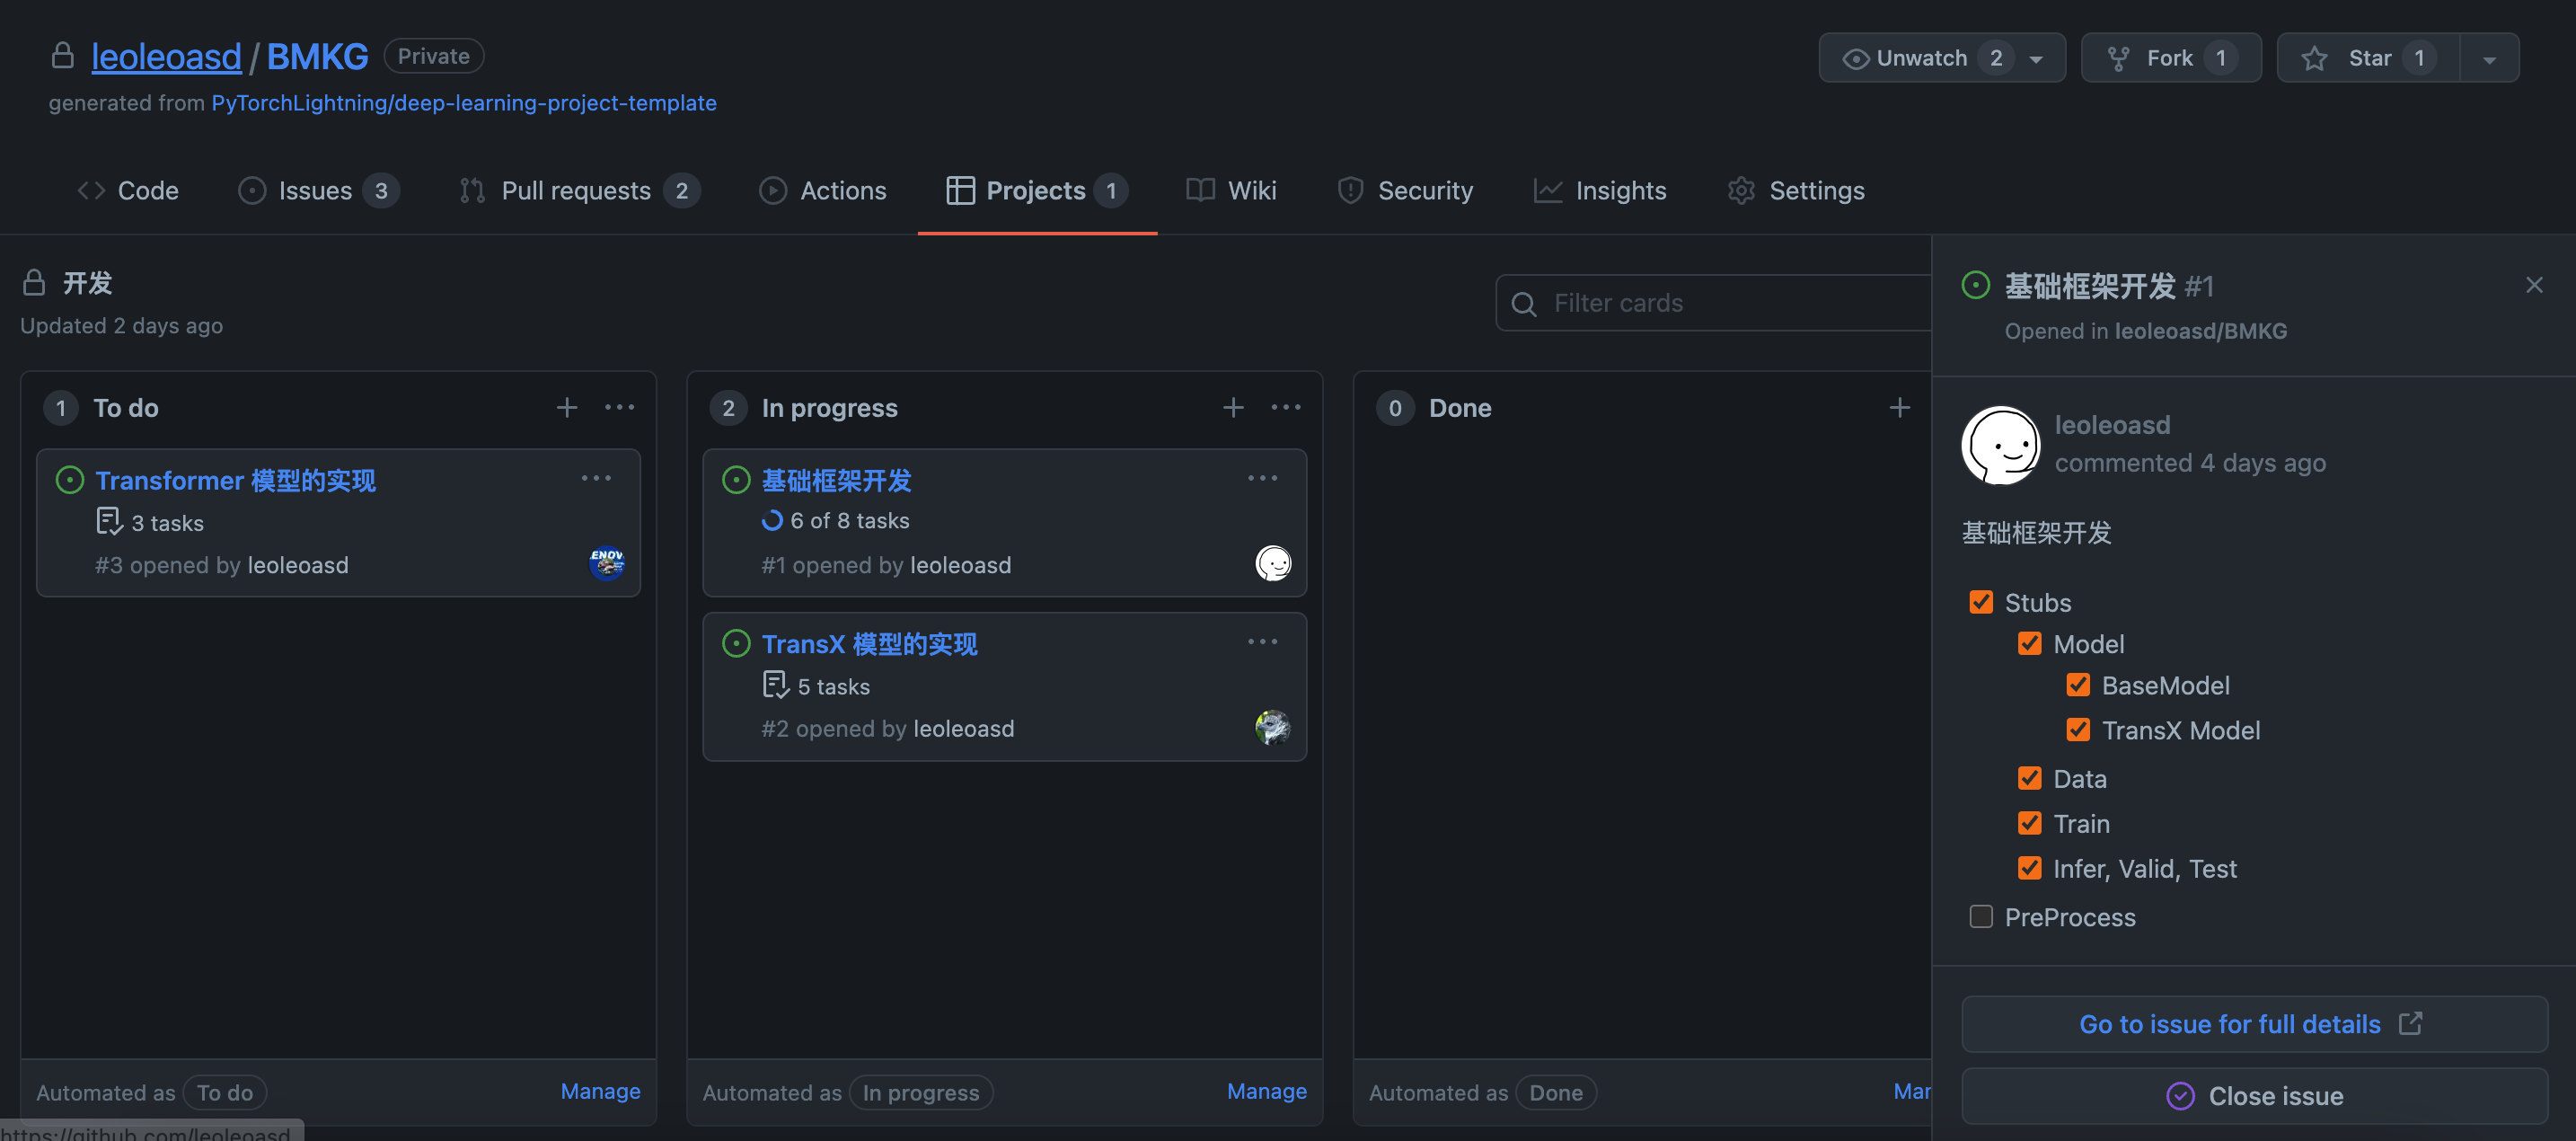
\includegraphics[width=.8\linewidth]{image2.png}
    \end{center}
    \begin{outline}
        \1 基础框架的 stubs 已经完成
        \1 正在开发数据预处理图分割部分
    \end{outline}
\end{frame}

\begin{frame}{开发流程}
    \begin{outline}
        \1 每个人在自己的分支开发 (dev/xxxx)
        \1 通过Pull Request合并进入主分支
        \1 合并前rebase master
            \2 \texttt{git fetch; git rebase origin/master}
    \end{outline}
\end{frame}

\section{技术选型}
\begin{frame}{C++ or Rust?}
    技术栈对比:
    \begin{center}
        \begin{tblr}{
            width = 0.8\linewidth,
            colspec = {X[c]X[c]}
        }
            \toprule
            C++ & Rust \\
            \midrule
            CPython & PyO3 \\
            numpy C-API & rust-numpy \\
            OpenMP & Rayon \\
            std::async & Tokio / std \\
            \bottomrule
        \end{tblr}
    \end{center}
\end{frame}

\subsection{Why Rust?}

\begin{frame}[fragile]{Why Rust?}
\begin{minted}[breaklines,fontsize=\footnotesize]{cpp}
PyMODINIT_FUNC PyInit_spam(void) {
    PyObject *m;
    m = PyModule_Create(&spammodule);
    if (m == NULL) return NULL;
    SpamError = PyErr_NewException("spam.error", NULL, NULL);
    Py_XINCREF(SpamError);
    if (PyModule_AddObject(m, "error", SpamError) < 0) {
        Py_XDECREF(SpamError);
        Py_CLEAR(SpamError);
        Py_DECREF(m);
        return NULL;
    }
    return m;
}
\end{minted}
\end{frame}
\begin{frame}[fragile]{Why rust? -- Cleaner Interface}
    \begin{minted}[breaklines,fontsize=\small]{rust}
create_exception!(bmkg, MyError, pyo3::exceptions::PyException);
#[pymodule]
fn bmkg(_py: Python, m: &PyModule) -> PyResult<()> {
    m.add("MyError", _py.get_type::<MyError>())?;
    Ok(())
}
    \end{minted}
\end{frame}
\begin{frame}[fragile]{Why Rust? -- Safer}
\begin{minted}[breaklines,fontsize=\footnotesize]{cpp}
PyMODINIT_FUNC PyInit_spam(void) {
    PyObject *m;
    m = PyModule_Create(&spammodule);
    if (m == NULL) return NULL;
    SpamError = PyErr_NewException("spam.error", NULL, NULL);
    Py_XINCREF(SpamError);
    if (PyModule_AddObject(m, "error", SpamError) < 0) {
        Py_XDECREF(SpamError);
        Py_CLEAR(SpamError);
        Py_DECREF(m);
        return NULL;
    }
    return m;
}
\end{minted}
\texttt{Py_XINCREF? Py_XDECREF? Py_CLEAR? Py_DECREF?}
\end{frame}

\begin{frame}[fragile]{Why Rust? -- Easy Async Programming}
    \definecolor{barblue}{RGB}{153,204,254}
    \begin{ganttchart}[
        % canvas/.append style={fill=none, draw=black!5, line width=.75pt},
        hgrid style/.style={draw=black!5, line width=.75pt},
        today rule/.style={
          draw=black!64,
          dash pattern=on 3.5pt off 4.5pt,
          line width=1.5pt
        },
        title/.style={draw=none, fill=none},
        title label font=\bfseries\footnotesize,
        include title in canvas=false,
        bar label font=\mdseries\small\color{black!70},
        bar label node/.append style={left=2cm},
        bar/.append style={draw=none, fill=barblue},
        bar progress label font=\mdseries\footnotesize\color{black!70},
        expand chart=\textwidth,
        bar height=.9,
        y unit chart=.5cm
      ]{1}{10}
      \ganttbar{Forward}{1}{2} \ganttbar{}{5}{6} \ganttbar{}{9}{10}\\
      \ganttbar{Backward}{3}{4} \ganttbar{}{7}{8}\\
      \ganttbar{Sampling}{4}{4} \ganttbar{}{8}{8}\\
    \end{ganttchart}
\end{frame}

\begin{frame}[fragile]{Why Rust? -- Easy Async Programming}
\begin{minted}[breaklines,breakbefore=.,fontsize=\footnotesize]{rust}
async fn heavy_task() -> PyResult<String> {
    println!("Doing heavy compute task...");
    // Sleep 2 seconds
    tokio::time::sleep(time::Duration::from_secs(2)).await;
    Ok(String::from("Hooray!"))
}
#[pyfunction]
fn negative_sampling_prepare(data: &PyDict, file_name: &str, partition: u32) -> PyResult<GraphPartitionResult> {
    let rt = Runtime::new()?;
    let handle = rt.spawn(heavy_task());
    Ok(GraphPartitionResult{
        rt,
        handle: Some(handle),
    })
}
\end{minted}
\end{frame}

\begin{frame}[fragile]{Why Rust? -- Easy Async Programming}
    \begin{minted}{python}
future = negative_sampling_prepare(...)
some_heavy_compute_task()
result = future.wait()
    \end{minted}
\end{frame}

\subsection{Some Concerns}
\begin{frame}[fragile]{Some Concerns -- Is it stable?}
    \begin{outline}
        \1 Is it stable? \pause
        \1 Yes! \pause
        \1 PyO3 的第一个Release发布于2017年
        \1 至今已有5年,文档、教程等资料非常丰富
    \end{outline}
\end{frame}
\begin{frame}[fragile]{Some Concerns -- Is it suitable for industrial usage?}
    \begin{outline}
        \1 Is it suitable for industrial usage? \pause
        \1 Yes! \pause
        \1 一个例子:
            \2 Huggingface 的 Tokenizer 包(于2020年开始开发)就使用PyO3
            \begin{tblr}{
                colspec={X},
                width=\linewidth
            }
            \vline[2pt, gray8]
                Extremely fast (both training and tokenization), thanks to the Rust implementation. Takes less than 20 seconds to tokenize a GB of text on a server's CPU.
            \end{tblr}
    \end{outline}
\end{frame}
\begin{frame}[fragile]{Some Concerns -- 环境好配吗?}
    \begin{outline}
        \1 环境好配吗? \pause
        \1 Yes! \pause
        \1 开发过程中调试代码:
            \2 安装 Rustup: \url{https://rustup.rs/} 一键安装
            \2 安装 maturin: \texttt{pip install maturin}
            \2 编译代码: \texttt{maturin develop -r}
            \2 实验室服务器已经安装好
        \1 发布pip包:
            \2 可直接编译二进制wheel发布
            \2 源码发布需要用户下载安装 Rustup
    \end{outline}
\end{frame}
\begin{frame}[fragile]{Some Concerns -- Maintainability?}
    \begin{outline}
        \1 如何维护 \pause
        \1 我会持续维护
        \1 清华本科的优秀同学应该都会Rust
    \end{outline}
\end{frame}
\begin{frame}[standout]
    Any Thoughts?
\end{frame}
\end{document}
